\section{Linux Network Stack}\label{sec:linux_net}

The previous sections have demonstrated how a malicious device can take over a machine; exploiting the buggy implementation of SBP-2. In this section we explore new attacks on the Linux network stack; where, \textit{Means} and \textit{Opportunity} are harder to come by. 
\subsection{\shinfo}
The sk\_buff is a common data structure that is used in the Linux network stack to hold information  representing a network packet and is used by all network card drivers. Struct \skb holds the metadata of a network packet e.g., its size, associated socket and device and other important information. One of these fields, is a pointer to a data buffer. The data is usually located on a separate page (see Figure \ref{fig:sh_info}). This  separation means that \skb is never (intentionally) mapped to the device; resulting in previous works \cite{thunder} declaring that the Linux network stack is not susceptible to DMA attacks. In reality, the Linux network stack supports packet cloning by copying sk\_buff metadata and letting the new one point to the same data as the old one\cite{drivers2005linux}. To support this data sharing, the \shinfo metadata structure is allocated as part of the data buffer and consequentially is always mapped to the device. Just as in the previous attack, \shinfo is unwittingly mapped for the device with the permissions of the packet i.e., write for RX packets, read for TX packets and in some cases both read and write for XDP/XSK \footnote{\url{https://www.kernel.org/doc/html/v4.18/networking/af_xdp.html}}. This design decision is the \oportunity the malicious device needs. Figure \ref{fig:sh_info} shows how a malicious device can take advantage of a \shinfo to mount an attack on the server with 4 simple steps:
\begin{enumerate}[label=(\alph*)]
    \item an RX \skb and its data buffer are allocated. The data buffer is DMA mapped for the NIC with write access (the write access is to the whole 4K page). 
    \item \textit{destructor\_arg} field in \shinfo is overwritten to point inside the mapped page. Now the \textit{destructor\_arg} is pointing to struct \uarg which is created by the NIC.
    \item \uarg has a callback pointer that is now pointing to the mallicious code that resides on the same page\footnote{In case of NX-bit, its a ROP gadget and a stack}.
    \item when \skb is freed the callback is invoked.
\end{enumerate}
This scenario assumes that the \kva of the mapped page(a.k.a \means) is known to the NIC and that \shinfo will not be overwritten by the CPU. We tackle both issues in this section.
\begin{figure}
    \centering
    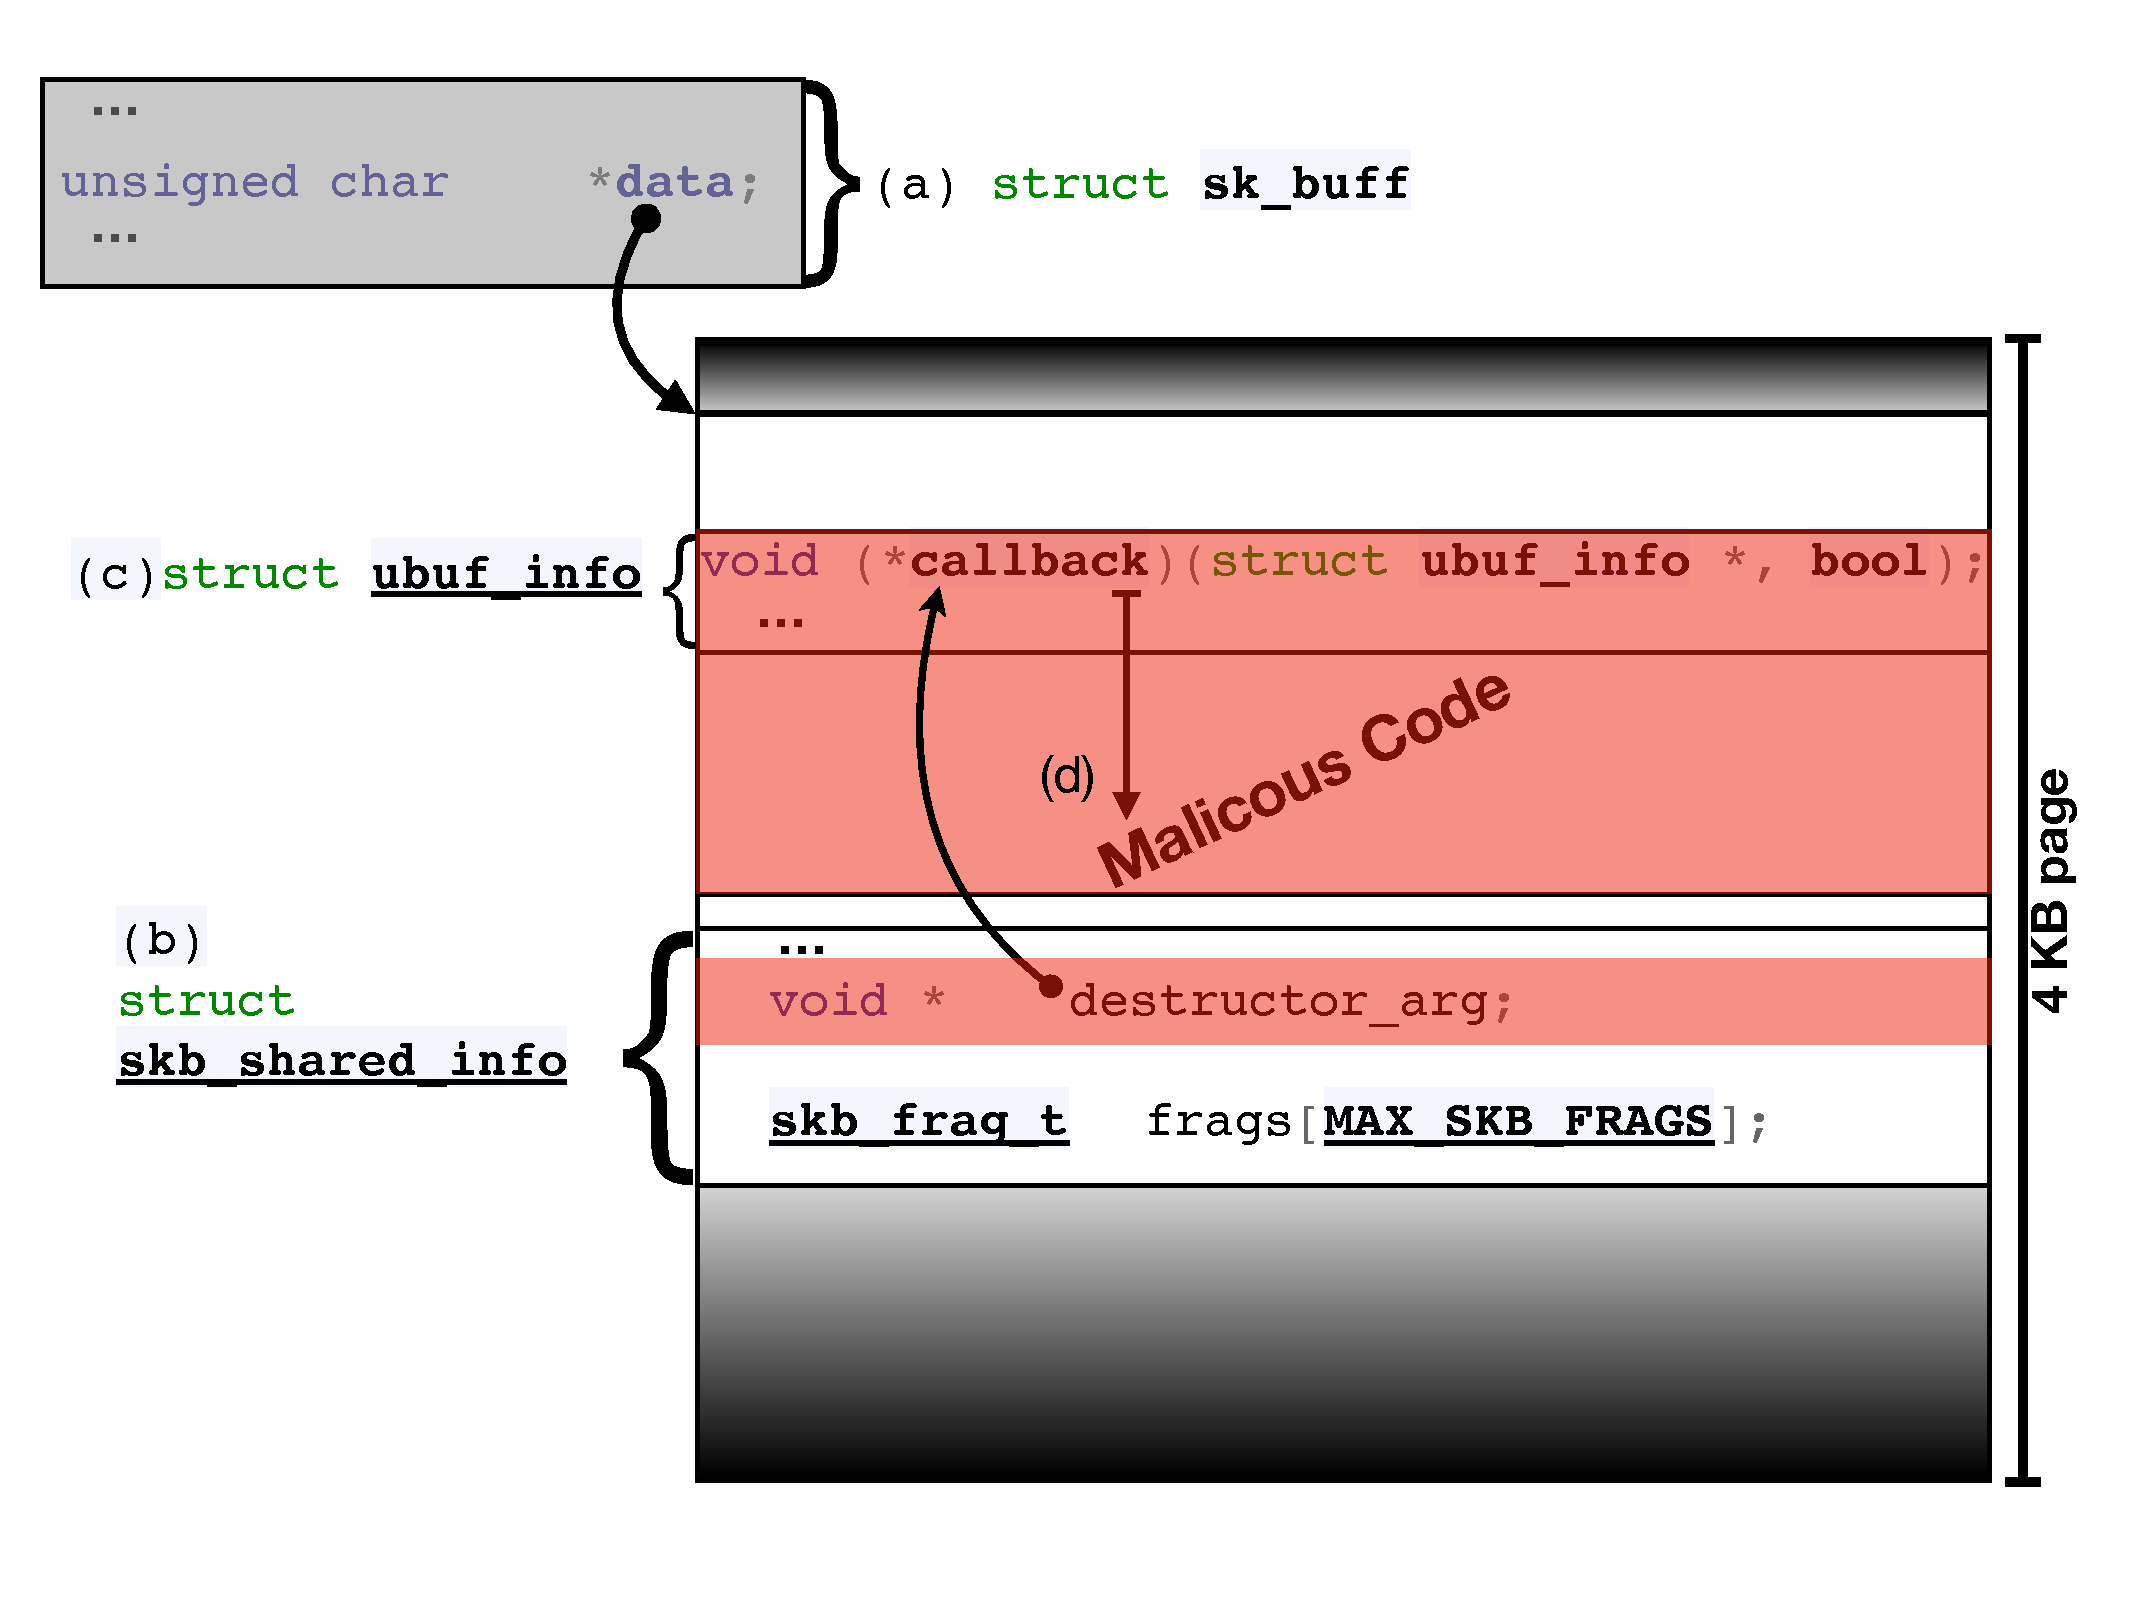
\includegraphics[width=1.2\linewidth]{figs/ubuf.pdf}
    \caption{Using \shinfo to run random code in kernel context.}
    \label{fig:sh_info}
\end{figure}

\subsection{Hacking \shinfo}\label{sec:shinfo}
Presumably, a correct use of DMA api by the device driver could easily thwart the attack outlined in Fig \ref{fig:sh_info}. Unmapping the buffer and then initializing \shinfo; should allow the CPU to undo any malicious changes the NIC may have perpetrated. As it turns out, multiple device drivers \footnote{A partial list appears in \ref{apndx:wrong_order}} first create an \skb and only then unmap. Many high speed drivers, avoid unmapping altogether due to the performance penalty of dma\_unamp \cite{MMT16,MSMT18}. These unmapping practices (or bugs) allow the NIC ample opportunity to execute an attack. But even when the order is correct \shinfo is not safe from modifications. The default iommu mode in Linux is deferred protection; and though the unmapp function was called in the right order, the device can still access it via the IOTLB. A security conscious admin may change the default setting to strict. Now the \iova the NIC had for that page is no longer valid. And yet the device can still modify \shinfo. The vulnerability stems from the way \data is allocated. An RX \skb is allocated via the \texttt{napi\_alloc\_skb} or \texttt{netdev\_alloc\_skb} functions\footnote{There are several other options as well, but the principle is the same. \url{https://elixir.bootlin.com/linux/v5.3.8/source/net/core/skbuff.c\#L519}}; these function use a page\_frag to allocate the \data buffer that contains \shinfo. Page\_frag is an efficient method for allocating small buffers of memory. A page\_frag is initialized by allocating a contiguous memory region(usually 32KB) and set a \textit{va} pointer to the end of the region; an allocation request for \texttt{B} bytes will subtract \texttt{B} bytes from the pointer and return the new value of \textit{va}. 
%\begin{comment}The page\_frag is local to each CPU so there is no contention; page\_frag is replaced with a new one when exhausted.\end{comment} 
This mechanism for memory allocation is very fast, but it also means that consecutive \data buffers will share memory pages. The NIC doesn't need to access the unmapped \iova to modify the \shinfo; it can use the \iova for the next data buffer. The lower 12 bits(the offset on the page) of the \iova  are the same as in the \kva, meaning that the NIC can easily know which \iova overlaps with the previous buffer. In figure \ref{fig:sh_info}, the shaded areas belong to the neighbouring \data buffers. It seems that the only way to secure \shinfo, is to never map it\cite{MSMT18}.

\subsection{Ring Flod}
In \ref{sec:shinfo} we have established that that a malicious NIC has ample opportunity both to create a ROP stack and alter a callback function that will use it. A NIC can calculate a valid kernel\_base pointer(as we have shown in \ref{sec:kaslr}) and other randomized base pointers just by scanning pointers leaked in TX packets\footnote{For example the NIC can spoof a constant stream of pings that will continuously leak kernel pointers}; thus circumventing KASLR. At this point the malicious NIC is still missing the \means to execute an attack.
While the NIC has a \mabaf and a callback function to override; it is missing the \kva to said buffer.
\begin{comment}
%Every RX packet is a possible buffer of malicious code, but the device is only given the buffer iova. The mapping between an iova and its kva is held in the device page table and the device driver meta-data; neither is accessible to the device. On RX the \texttt{struct page} address is filled by the driver(not the KVA) and additionally while we have write access we don't have read access. This means that while the \page address is in a mapped page; we cant read it because its write only. If we could read the \page address; we still wouldn't have the KVA. \newline 
%Luckily for the attacker, the current memory model of x86-64 and ARM Linux servers is SPARSEMEM\_VMEMMAP \cite{mem_model}. Under this memory model the transition between KVA,PFN and \page is trivial once we have the vmem\_base value (Fig \ref{fig:mem_model}). We can guess the value of vmem\_base by looking for kernel pointers in pages mapped for TX packets.\newline
\end{comment}
\newline
The boot process is deterministic; executing the same set of commands, initiating the same modules and allocating the same amount of memory each reboot. While the actual pages each module gets will vary in a multi-core machine due to timing issues, the drift is not expected to be to large. We evaluate this assumptions on a DELL 730 server equiped with a ConnectX-5 NIC, running 256 reboots on Ubuntu 18.04 with kernel 5.0. \textcolor{magenta}{different kernel versions could be better, and three Dell machines}. In the fig\footnote{\textcolor{red}{Please generate table of RingFlod Results}} we show the memory used by each driver and how many of the PFNs repeat in more than 50\% percent of reboots. \textcolor{magenta}{Need to see If we can improve this number}. Thus an adversary that has some knowledge about the physical setup and the kernel version can guess with a high probability a valid \kva for one of the RX pages. Whats left is to fill all the pages with a valid \mabaf and execute an attack as shown in \ref{fig:sh_info}. The callback wont necessarily point back to its own page; but rather to any of the 14K such pages on a 28 core machine\footnote{We assume 1.default RX ring with 1K entries 2.MTU of 1500 where each page is shared by two skbs}. The probability of this attack depends on the driver version and NIC capabilities.For example ,some NICs have a HW LRO capability; where a NIC can aggregate multiple TCP packets into a single TCP packet, larger than MTU (bnx2x and mlx5)\footnote{\textcolor{red}{need reference to capability}}. Drivers configured with these options have a much larger memory footprint and as a result easier to target with a RingFlod attack.  

\subsection{Privilege escalation}
\begin{figure*}
    \centering
    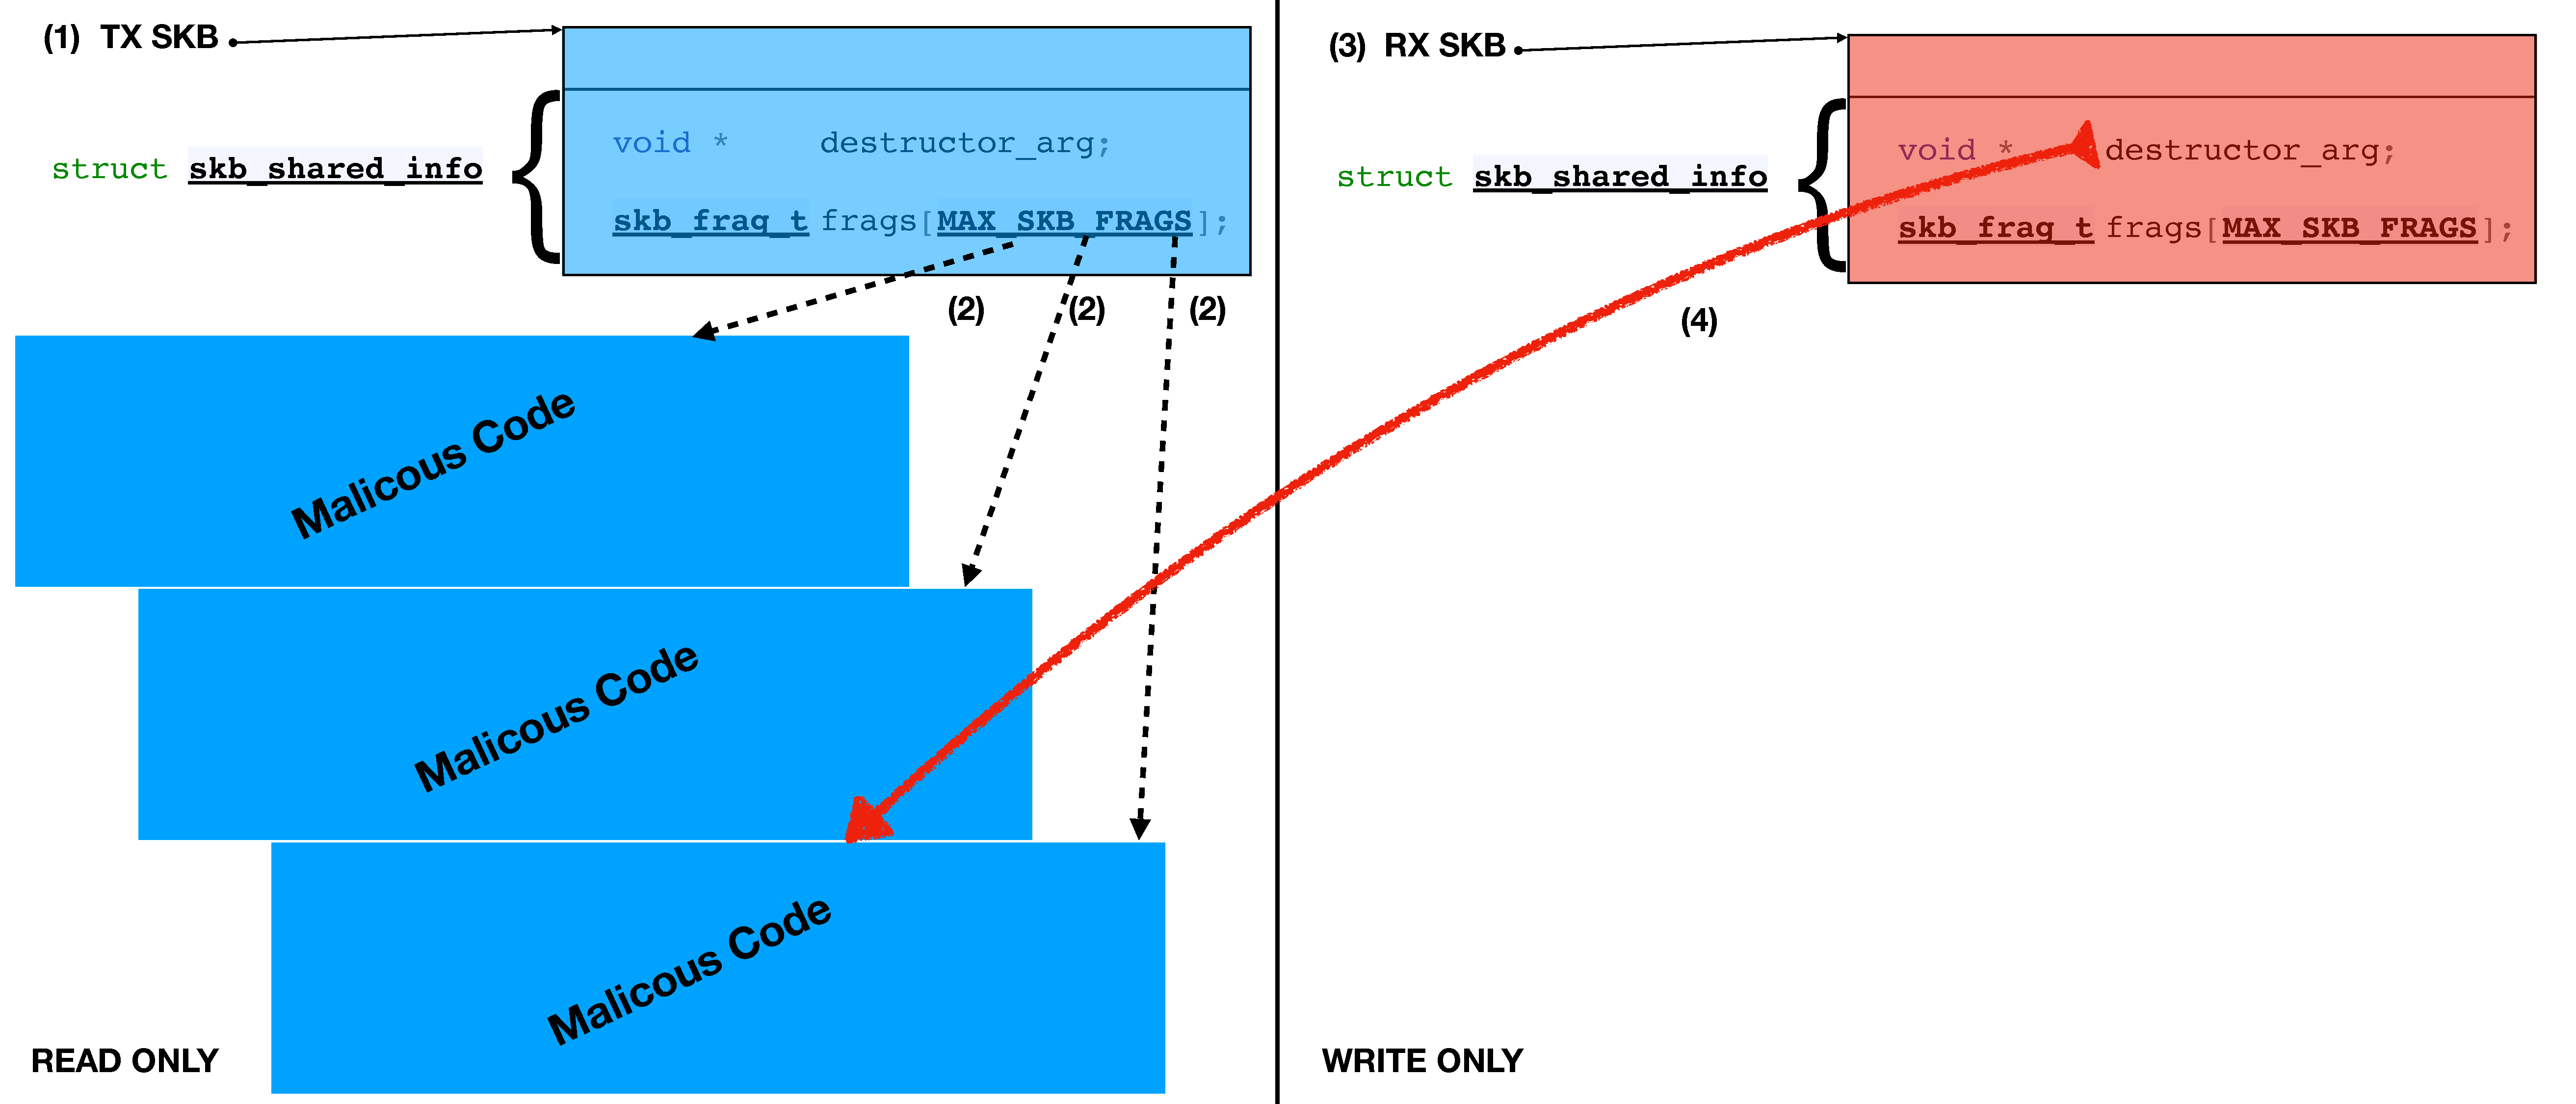
\includegraphics[width=1.1\linewidth]{figs/paylopad_both.pdf}
    \caption{An sk\_buff filled with malicious code}
    \label{fig:payload}
\end{figure*}
\shinfo of a TX packet is read only to the NIC.
But if the fragments hold malicious content; its all the malicious NIC needs for a successful attack. The readable \shinfo holds a \kva for a \page. This both allows the NIC to break KASLR and gives a \kva\footnote{\textcolor{magenta}{Do show exactly what are the KASLR bits and how you break it}} of a valid \mabaf. To implement the attack the NIC will generate an RX packet and fill the \uarg address from the calculated \kva.
The NIC will hold off on the TX completion event in order to make sure that \kva is not freed by the TX completion handler; before the poisoned RX packet is processed. A TX completion event that fails to appear in due time, will trigger a TX T/O error that will flush all buffers; the T/O is set by the driver usually to 5 seconds, which is enough to implement an attack.\newline
In this scenario the attacker doesn't need any prior knowledge of the kernel or the hardware. The only assumption is that there is an accomplice (witting or unwitting) that can open a socket in user-space. For that matter even in user-space of a guest machine; making any cloud VM a valid intrusion tool.

\subsection{Packet Forwarding}
Packet forwarding functionality is usualy disabled by default in Linux machines. But some Linux servers may function as a router or a load balancer; these machines will have packet forwarding enabled. In this scenario the NIC can independently generate an RX packets with a \mabaf. These packets can have valid 5 tuples to their network. The driver will complete the \page address of the buffer. \textcolor{red}{These packets will be forwarded and so become a TX packet that can be used as described in the previous attack.} \footnote{Need to check what happens to sh\_info, can we just forward a packet with frags (MTU, is usually a limiting factor)}

\begin{figure*}
    \centering
    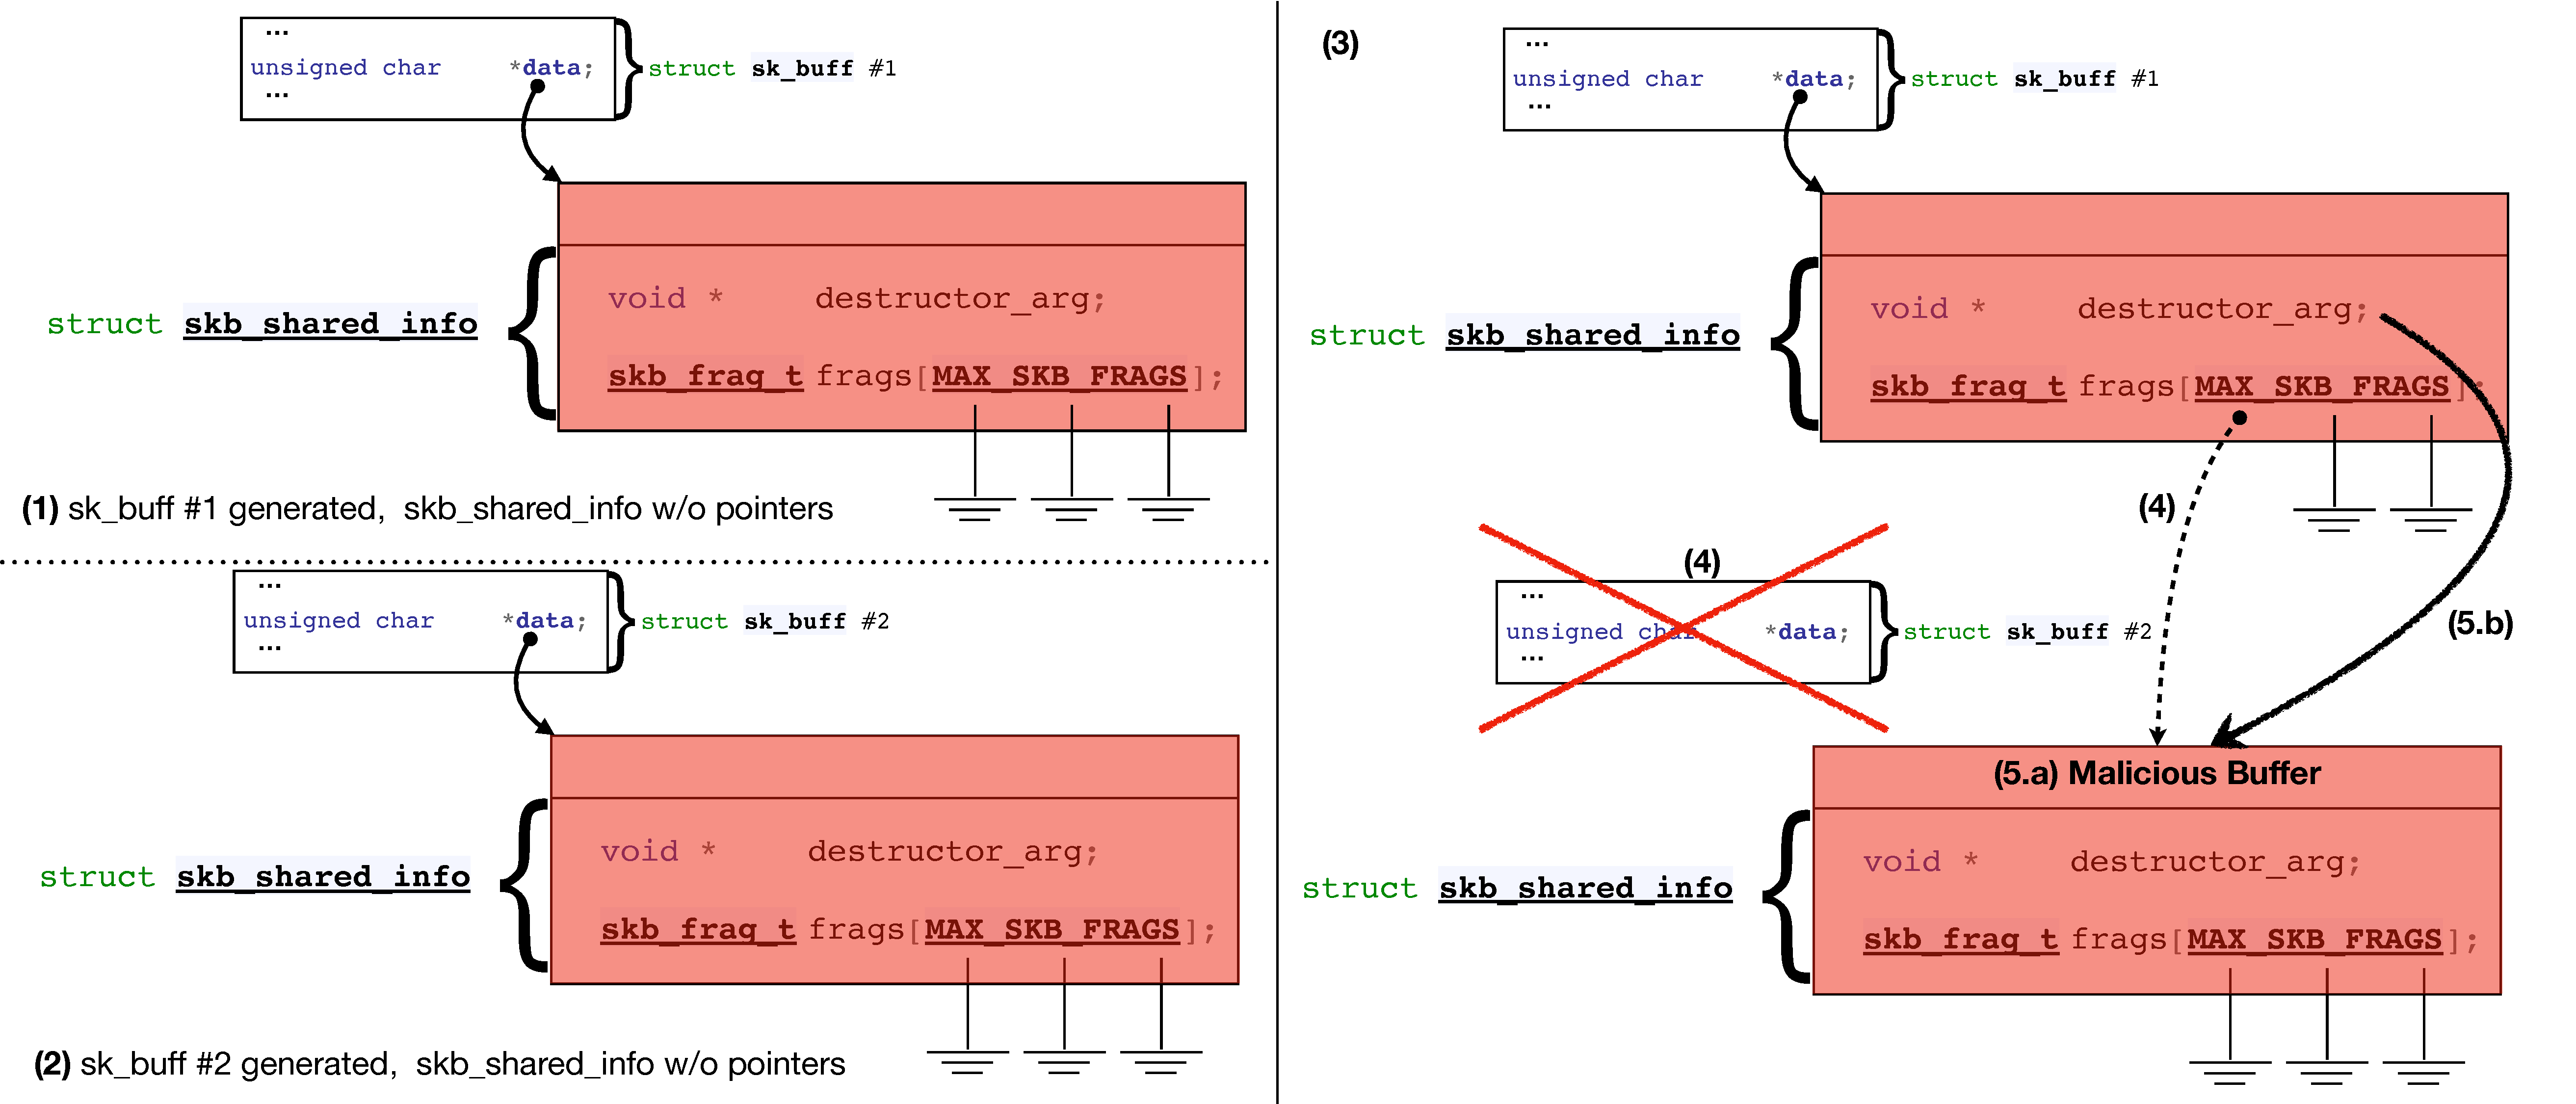
\includegraphics[width=1.1\linewidth]{figs/gro_generation.pdf}
    \caption{An sk\_buff filled with malicious code}
    \label{fig:gro}
\end{figure*}

\subsubsection{When page frags are used indiscriminately}
\textcolor{magenta}{Unfortunately the following is not found in nature... - XDP Does :)}\newline
In case where both TX and RX sh\_info come from the same page frag. The NIC can read arbitrary kernel addresses by modifying the frag list of a TX skb thus making the driver map random addresses.
Being able to read the \shinfo, allows the NIC to generate an RX packet packet with \mabaf; the \kva of which will be written by driver and read by the NIC via TX iova. From this point and on we refer the reader to the steps in the previous sections.
\subsection{XDP}
\textcolor{red}{XDP (5.1.12)is not umpapping or using DMA\_MAP\_BIDIR \- please show its ill advised...} \textcolor{magenta}{The linear skbs in mlx5 are mapping sh\_info as BI\_DIR, need to see when linear used vs non-linear and to check othe XDP drivers. When sh\_info is mapped BI\_DIR its all we need to attack.\newline
It seems linear skb (No (HW?)LRO and MTU<1500 : verify with experimnt or Boris) means no frags, while \begin{enumerate}
    \item build\_skb is used on a mapped page
    \item page is unmapped in a deferred way, regardless of iommu policy; a driver hack.
\end{enumerate} 
we cant take advantage from driver writing the \page address :( (We still can benefit from RingFlod, Escalation, Forwarding(non linear, pending experiment)). What we can do is look into \begin{enumerate}
    \item skb\_try\_coalesce
    \item SW LRO/GRO
\end{enumerate}}.
\newline
\textcolor{magenta}{In addition reviewing other drivers for the intersection of DMA\_BIDIR \^ (skb\_add\_rx\_frag||skb\_fill\_page\_descriptor)}